% Title:    A LaTeX Template For Responses To a Referees' Reports
% Author:   Petr Zemek <s3rvac@gmail.com>
% Homepage: https://blog.petrzemek.net/2016/07/17/latex-template-for-responses-to-referees-reports/
% License:  CC BY 4.0 (https://creativecommons.org/licenses/by/4.0/)
\documentclass[10pt]{article}

% Allow Unicode input (alternatively, you can use XeLaTeX or LuaLaTeX)
\usepackage[utf8]{inputenc}
\usepackage{hyperref}
\usepackage{xcolor}
\usepackage{todonotes}

\usepackage{microtype,xparse,tcolorbox}
\newenvironment{reviewer-commentX}{}{}
\tcbuselibrary{skins}
\tcolorboxenvironment{reviewer-comment }{empty,
  left = 1em, top = 1ex, bottom = 1ex,
  borderline west = {2pt} {0pt} {black!20},
}
\ExplSyntaxOn
\NewDocumentEnvironment {response} { +m O{black!20} } {
  \IfValueT {#1} {
    \begin{reviewer-commentX}
      \setlength\parindent{2em}
      \noindent
      \ttfamily #1
    \end{reviewer-commentX}
  }
  \par\noindent\ignorespaces\color{blue}
} { \bigskip\par }

\NewDocumentCommand \Reviewer { m } {
  \section*{Comments~by~Reviewer~#1}
}

\NewDocumentCommand \Editor { m } {
  \section*{Comments~by~Editor}
}

\NewDocumentCommand \ToolComments { m } {
  \section*{Tool~Comments~by~Reviewer~#1}
}

\ExplSyntaxOff
\AtBeginDocument{\maketitle\thispagestyle{empty}\noindent}

% You can get probably get rid of these definitions:
\newcommand\meta[1]{$\langle\hbox{#1}\rangle$}
\newcommand\PaperTitle[1]{``\textit{#1}''}

\title{Response letter to EMISAJ Manuscript entitled "Multi-level modeling with Openflexo/FML- A contribution to the MULTI process challenge"}
%\author{Author1 \and Author2 \and Author3}
\date{\today}

\begin{document}

Dear Editor,

\bigskip
Thanks for your message of August 16th, 2021, in which you suggested preparing a revision of our manuscript  \textbf{Multi-level modeling with Openflexo/FML- A contribution to the MULTI process challenge}. 

\bigskip
We are grateful to the reviewers for their interest, effort, and suggestions. We detail in the following pages how we have addressed the reviewers' concerns; we are confident that the paper is now improved, and hope that you will agree. We have organized the responses to the comments on a per-reviewer basis, focusing, as suggested, on: 

\begin{itemize}
\item Improving the presentation.
\item Provide a more explicit description of how the multi-level modelling emulation is achieved.
\item Discussing the general advantages and limitations of the multi-level emulation, including a clarification of what the implications would be of supporting more "levels" than the challenge required.
\end{itemize}

Moreover, the paper has been thoroughly revised to fix minor issues and to give the additional clarifications required by the reviewers. Please let us know if you need any further information or clarification.

\bigskip
Sincerely yours,

\bigskip
Sylvain, Guillaume, Caine, Joel, Jean-Christophe, Salvador, Fabien and Antoine

\pagebreak

\Editor{}

\begin{response}{the reviewers have made suggestions for improving the presentation but also raised a number of issues requiring clarification. An overarching theme is the request for a more explicit description of how the multi-level modelling emulation is achieved and what its general advantages and limitations are, including a clarification of what the implications would be of supporting more "levels" than the challenge required.} 

We have been more explicit to explain how we use the FML language at the end of the introduction, and in various figures. TODO.


\todo[inline]{We have enhanced the presentation of both, Openflexo/FML and our solution to the challenge so that: 1) the techniques we use to \emph{achieve} multi-level capabilities are more explicit; and, 2) the advantages and disadvantages of using them in order to fulfil the challenge requirements become clearer. Notably, we have added many details in the final paragraphs of the introduction section, improved the Section 2, devoted to the description of OpenFlexo, refactored figures X, Y, Z.}
\end{response}


\begin{response}{We very much welcome a "conventional" response to the challenge but would like to see the respective reviewer questions addressed in a revised version which is explicit as possible about the advantages and the disadvantages of the emulation. You may find the references listed below useful to keep explanations concise by referencing related work (note that reviewer 3’s “Type-Instance pattern” is also known as the “Type Object” pattern). You should also respond to other concerns reviewers raise, either by making changes to the submission or in the form of an authors' response.} 
The related work section has been modified to show that we are not the first conventional response with multi-level emulation, and to improve comparisons and limitations of different approaches.\todo[inline]{I do not understand this answer. We are saying that other approaches are also unconventional?}
\end{response}


\begin{response}{Finally, to achieve consistency with other submissions, could you please change the subtitle to "A Contribution to the Multi-Level Process Challenge"?}

Done.
\end{response}

\pagebreak

\Reviewer{\#1}
\begin{response}{In section 2 Technology the authors describe the foundations of the Openflexo approach. Here it would greatly help the reader to see an example how the approach works for traditional modeling languages. For example, how would you realize a small subset of BPMN with the approach? This could briefly be illustrated so as to give the reader an immediate understanding. Especially, the 'metamodel'-agnostic approach seems very interesting but I would like to see how that is used for traditional modeling approaches.}

The Figure \ref{fig:BPMNSubsetExample} (above) shows how to realize a small subset of BPMN with Openflexo/FML (assuming a metamodel of the full specification of BPMN exists). Concretely, we show  how a VirtualModel (SimplifiedBPMN) can filter an existing model (BPMN) and be instantiated. Note that connection with external sources is not required for our solution to the challenge and is only represented in order to illustrate the capabilities of Openflexo/FML. Therefore, in the article we choose not to give this level of details and focus on the left part of the figure. 

\todo[inline]{I've refactored the paragraph above. To be verified.}

\begin{figure}[t]
    \centering
    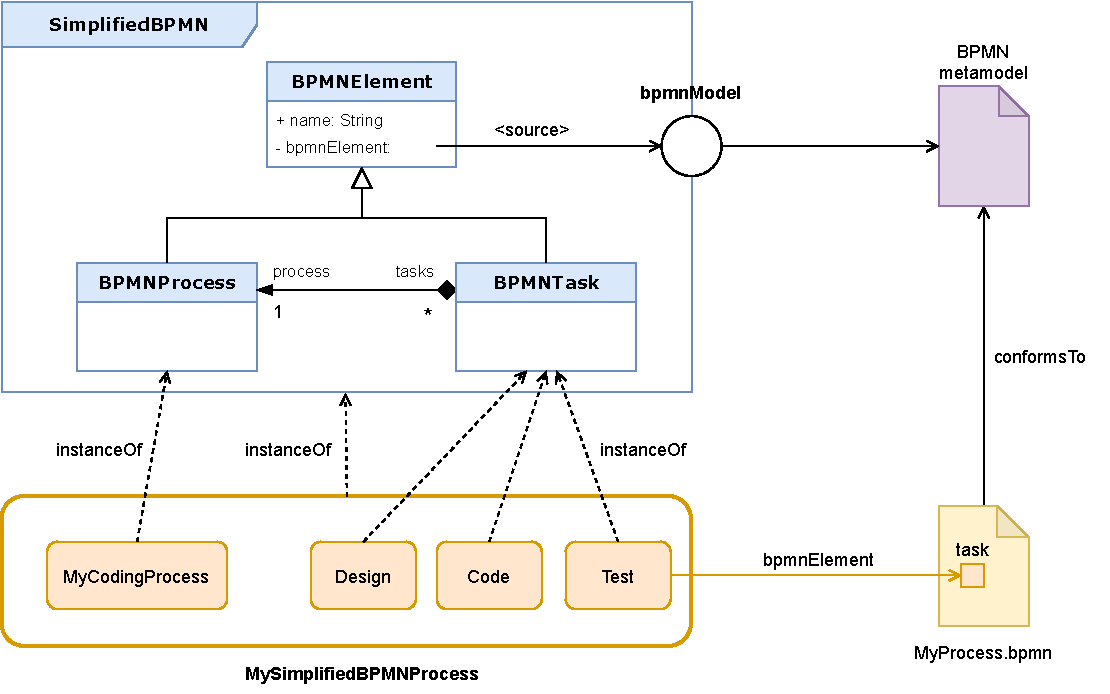
\includegraphics[width=1.0 \textwidth]{Figures/BPMNSubsetExampleWithExternalConnexion.pdf}
    \caption{An example of BPMN subset built on top of a BPMN/EMF model}
    \label{fig:BPMNSubsetExample}
\end{figure}

%\begin{lstlisting}
%use org.openflexo.technologyadapter.emf.EMFModelSlot as EMF;
%import ["http://www.omg.org/spec/BPMN/20100524/MODEL-XMI"] as BPMN_METAMODEL;
%
%// A simplified BPMN metamodel exposing
%// both concepts BPMNProcess and BPMNTask
%model SimplifiedBPMN {
%
%  // Connexion to a .bpmn file
%  EMFModel bpmnModel 
%    with EMF::EMFModelSlot(
%        metaModel = BPMN_METAMODEL);
%
%  // Abstract concept BPMNElement defining
%  // a name and a link to an eventual BPMNElement
%  // in .bpmn file
%  abstract concept BPMNElement {
%  	EMFObjectIndividual bpmnElement 
%  	    with EMF::EMFObjectIndividualRole (
%			source = bpmnModel
%		);
%    String name values bpmnElement.name;
%  }
%
%  concept BPMNProcess extends BPMNElement {
%
%    // Describe here properties and
%    // behaviours for BPMNProcess concept
%    ...
%
%    concept BPMNTask extends BPMNElement {
%
%        // Describe here properties and
%        // behaviours for BPMNTask concept
%        ...
%
%    }
%
%    // Other core concepts
%  }
%}
%\textbf{}\end{lstlisting}

\end{response}

\begin{response}{Also, at the stage of section 2, the characterization of the FML language should be made clearer. The metamodel in Figure 2 seems mainly conceptual - but at the same time you refer to it as a basis for implementation. Could that be clarified? eg you have the class "Behavior" - which is a concept and I did not understand right away what it is composed of. On the other hand you have for example the class "ModelSlot" which seems like a very technical realization. Also, you note that roles have types but I could not find any types in the metamodel (?). Thus, I propose to include a more detailed version of your metamodel at this stage. Please note that EMISAJ does not have a page limitation, so no worries if that should require more space.} 
We've changed figure 2. It shows \texttt{Type} and the main concepts used by FML. TODO. Explanation of figure has been improved. 
\end{response}

\begin{response}{In Figure 5, the base metamodel for representing processes is shown - however it is not linked to the concepts you introduced before. Would it be possible to maybe graphically highlight how it relates to the metamodel in Figure 2? Besides, as multi-level modeling is much different to traditional modeling, you may want to consider using a different notation rather than UML class diagrams - as these are commonly known for traditional modeling approaches. When reading the paper, I actually marked the references to types in yellow in my copy - ie from ProcessType to TaskType and from ActorType to ActorType (on the attribute levels) - this helped me to see more clearly where you have references from attributes to types - but that's just my way of doing it.} 
TODO. Faire le lien entre figure 2 et les représentations des figures 3, 4, 5, 6 et 7. Package = VirtualModel, Classes bleues = FlexoConcept, attribut =(~) Get/GetSetProperty, association = FlexoRole, no FlexoBehavior visible. (!! Dans la figure 2 il n'y a pas d'héritage possible visible entre FlexoConcept.) Le niveau orange est l'instantiation / interprétation du FML.
\end{response}

\begin{response}{Regarding Figure 6 and Figure 7: In Figure 7 you show the process incl. sequence connectors - however in Figure 6 these seem to be missing - maybe to reduce complexity? I would suggest to probably focus on a subset of the process from Figure 7 and also show how the connectors are realized. To me this would increase the comprehensibility / consistency. Ie I could then infer exactly, how elements from the concrete model have been realized in the background.} 
TODO.
\end{response}

\begin{response}{in Figure 9 you show the model editor. Could you please also add a screenshot of the metamodel editor?} 
TODO.
\end{response}

\begin{response}{There are some minor typos throughout the manuscript (eg also regarding the reference Jeusfeld2019; choose -> chose; axis -> axes; aN FML virtual model...; etc.)} 
TODO.
choose $\rightarrow$ chose OK ; axis $\rightarrow$  axes OK ; je ne comprends pas pour Jeusfeld2019
(deeptelos2019) ni pour aN FML (je dirais ``a FML'', mais je puis me tromper)
\end{response}


\pagebreak

\Reviewer{\#2}

\begin{response}{The basic idea of model federation is interesting, its primary focus is not on creating multi-level models. However, as the approach is quite flexible, multi-level behavior can be emulated by model federation. This fact is possibly the most serious advantage and disadvantage of the paper at the same time. Advantage, since it brings us a completely new, different way of thinking, and disadvantage since it does not really help in categorizing/unifying multi-level methods and – for me – it also feels a little bit off-topic in this special issue. At this point, it should be mentioned that the authors managed to cover/solve all requirements of the challenge, thus the paper, as a solution to the challenge fits well.} We introduced at the end of the introduction a description of our approach. In a word, we use FML (linguistic level) as a tool to build models and meta-models that allows multi-level modelling. The evolution of models (multi-levels) is encoded as a hierarchy of models and meta-models. We do multi-level modelling on demands, and propose an organization guided by models evolution. 
\todo{Answering this is going to be tricky!}
\end{response}

\begin{response}{The paper gives us a short introduction (somewhat overlapping with the abstract, even at the level of sentences) and then the technology is detailed. The section is a bit hard to understand at first, the difference and the relationship between federated and virtual models could be explained in more detail especially considered that the challenge solution uses virtual models only. It is not clear, how federation works in this case.} 
We have improved the description and we hope this is much clearer. TODO.
\end{response}

\begin{response}{The third section contains an overview of the solution. Here, virtual models are instantiated to virtual model instances conforming to the virtual models acting as the metamodel for the virtual model instances. The question naturally arises: how does it work, if we have more abstraction levels?  In this section, the authors also discuss linguistic and ontologic instantiation. The explanation refers to Section 4 resulting in a hardly understandable analysis of different instantiation methods. Figure 4. does not help in clarifying the concepts either (e.g. using the name InstanceInstance seems to be a very bad decision). From the point of the muli-level behavior of view, the interpretation of the instantiation relationship is the most crucial one that is why this section must be clarified. Where are the rules of ontological instantiation defined, how are they enforced? The text mentions the (linguistic) instantiation mechanism of the FML Language… how does it work exactly?} 
We hope we have improved the explanation. \texttt{InstanceInstance} has been replace with \texttt{ObjectInstance}. TODO.
\end{response}

\begin{response}{Section 4 elaborates the solution in detail. Figure 5 presents an overview of the model elements handling P1 to P19. The diagram uses a UML-like annotation, which helps in making it understandable, but it also has a strange decision: roles (attributes) having a modeled concept as their type are visualized by links, but instead of using rolenames on the links, the concepts (classes) contain them. I strongly suggest following the UML guidelines here and use rolenames (similarly to multiplicity).}
TODO.
\end{response}

\begin{response}{Overall, the solutions for the requirements are correctly presented in this section, but there are some spots not clear enough. E. g. regarding ontological instantiation, the solution uses two kinds: single and multiple. More details would be welcome to see, what their exact semantics are and where do we enforce these semantic rules (is it enforced by the engine? Is the semantic hard-coded?). What are the contexts of the constraints (to which concept are they attached to)?} 
TODO.
\end{response}


\begin{response}{In Section 4.1.2 a behavior called newProcess is defined. Is it called automatically (by the framework) when creating a new process, or should the users call it? Is this a convention, or are such methods configured somehow to replace the usual constructors? According to the text, “same pattern applies” in several cases, but these patterns could be also included, because it is not completely clear to what part of the behavior “same” refers. In same cases, the diagram uses “/type”, while in the code it is “type” – why? The specialization of Actors is encoded by FML, wouldn’t be easier to use the built-in specialization instead?} 
TODO.
\end{response}


\begin{response}{In Section 4.2 it is mentioned, where the solution uses linguistic instantiation, but it is not clear by which component it is handled and what rules are followed when instantiating the concepts. In Section 4.3, tooling is elaborated. I suggest removing redundant information about the two editors and add more details on how the concrete syntax (e.g. the texts in the box of Fig. 9.) is defined.} 
TODO.
\end{response}

\begin{response}{In Section 5, the meaning of the category Conceptualization is hard to understand, does this mean that a concept is created that covers the requirement completely? In the case of ontological instantiation, the term “dual concept nature” and “instance nature” is mentioned… what do these terms mean?} 
TODO.
\end{response}

\begin{response}{Section 7 contains a rather short elaboration on related approaches. Although I agree that it is enough to focus on previous solutions here, much more detail and a comparison would be required.} 

We have extended Section 7. It discusses now previously published solutions to the challenge in more detail. Comparisons with our approach have been also extended.

\end{response}

\begin{response}{As Section 6 shows, the authors know exactly, why their solution may have difficulties as a multi-level modeling approach despite solving the given challenge. The solution is basically a smart, two-level modeling solution of the MULTI challenge. Multi-level behavior is emulated by constraints and additional mechanisms particularly written to this challenge. The result is a working workbench fulfilling the requirements but having limited reusability and extensibility. For example, it would be hard to increase the number of abstraction levels as class-like and object-like concepts are handled differently. Another problem may arise if we would use the framework as a prototyping tool and change the metamodel and the models at the same time.} 
TODO.
\end{response}

\begin{response}{Minor issues/questions:} 
\begin{itemize}
    \item Are there any tools supporting model federation besides Openflexo?
    \item Section 2. “In contrast to approaches that compose metamodels into a single large metamodel \item grouping all needed entities,…” - I do not see, why this is relevant here
    \item Figure 5 – concept Sequencing – the roles “in” and “out” are not represented by lines… why?
    \item What does the term “sub-concept” mean exactly? Please explain it before the first use
    \item ProgrammingLanguage concept is an enumeration… how is it modelled?
    \item “The Acme metamodel also defines a specialized task type Coding” – isn’t it CodingTask?
    \item “The value of the property producedArtifactTypes” – is it property, or role?

\end{itemize}
TODO. \todo{The idea is to group all the answers to the minor questions here.}
\end{response}


\pagebreak

\Reviewer{\#3}

\begin{response}{(1) The Type-Instance pattern is key to the authors approach to the challenge. However, the benefits of this pattern are not explored in the context of MLM. For example, the authors do not really explain approaches such as Clabjects or potency levels as they compare to the Type-Instance pattern (or the challenge). Why it the pattern better? Is it just a different approach? What can it do that other approaches cannot? Perhaps the benefit is that the Type-Instance pattern can be implemented in most modelling and implementation technologies whereas other approaches need special facilities? Finally, in terms of the pattern, why should anyone care - why would should they use the pattern?} 
TODO.
\end{response}

\begin{response}{(2) In section 1 the authors list 2 key reasons why a strict approach to modelling is sub-optimal. However, they do not establish the case that their approach uses these 2 features to any concrete benefit. It would be appropriate (perhaps at the end of the article) to revisit these features and to clearly demonstrate that their approach supports them and that they have concrete utility in some way in the context of the challenge.} 

We have added a paragraph in the Conclusions section indicating how Openflexo/FML permitted us to overcome the mentioned limitations of the strict modeling paradigm and how this was used in order to build our solution to the Multi-Level Process challenge. Notably, we mention how the type/object pattern allowed us to use model element instances as types in order to achieve ontological instantiation.
\end{response}

\begin{response}{(3) One of the key benefits of the Type-Instance pattern is that it provides a 'hook' on which semantics can be defined using constraints. There is a reified relationships between a type and its instance and therefore conditions can be defined that establish both static and dynamic semantics. I am confused regaring why this is not a key feature of the semantics for the challenge as it is implemented by the authors. Constraints are provided very sparingly compared to implementation of behaviour in FML. Unfortunately, since the dynamic semantics of FML is not provided (and is bespoke) this is less clear than it might otherwise be for the reader. Perhaps it would be better to use constraints in the context of the Type-Instance pattern to specify semantics? It would be more abstract than the current 'method' style semantics.} 
TODO.
\end{response}

\begin{response}{(4) Section 6 lists a number of benefits of the approach. Unfortunately, the presentation in the section is very general and none of the claims are justified in terms of concrete descriptions and/or examples. This section seems to be very important and could be of great interest to the reader. Perhaps it would be appropriate to reduce some of the rather implementation heavy descriptions earlier in the paper and increase the analysis in this section? In addition section 4.3 notes that MLM is key to the ability of Openflexo to create tooling. Again, this is very interesting, but no concrete details are provided as to how Openflexo uses the level agnotic features of the models to create tools. Can the essence of this be captured for Openflexo and then described in terms of how it facilitiates the tooling arising from the challenge?} 

We tried to illustrate subsections of section 6 by giving examples, by referencing figures and sections.

Concerning the fact that "MLM is the key to the ability of Openflexo to create tooling", the reviewer probably read "MLM" instead of "FML" (Flexo Modeling Language).
\end{response}

\begin{response}{(5) The paper makes an issue of the model federation approach supported by Openflexo, including the use of model slots. However, after introducing these concepts they do not seem to be important to the rest of the article. Perhaps this is an implementation concern that could be elided as its inclusion does not seem key to the contributions of the article. } 
TODO.
\end{response}

\begin{response}{Some minor issues:

(a) In fig 5: why are the in/out gateway features shown as properties and not as associations?

(b) On p. 7 'specialization' -> 'specializations'.} 
TODO.
\end{response}


\end{document}

